\documentclass{article}
\usepackage{amsmath, sfmath, multicol, tkz-euclide, array, enumerate, tcolorbox, tabularray, tipa}
\renewcommand{\familydefault}{\sfdefault}
\setlength{\parindent}{0cm}
\pagestyle{empty}
\usepackage[left=1in, top=0.5in, right=1in, bottom=0.5in]{geometry}
\tikzset{>=stealth, label style/.append style={font=\footnotesize}}
\tcbset{colback=white}

\newcounter{example}[section]
\newenvironment{example}[1][]{\refstepcounter{example}\par\medskip
   {\color{red}\textbf{Example~\theexample. #1}}}{\medskip}

\newcommand{\arc}[1]{%
    \setbox9=\hbox{#1}%
    \ooalign{\resizebox{\wd9}{\height}{\texttoptiebar{\phantom{A}}}\cr#1}}

\begin{document}

\section*{Areas of Circles and Sectors}

\begin{tcolorbox}[colframe=orange!70!white, coltitle=black, title=\textbf{Today I Can}]
\begin{enumerate}
    \item Find the area of circles, sectors, and segments of circles. 
\end{enumerate}
\end{tcolorbox}
\smallskip 

\begin{tcolorbox}[colframe=black!20!white, opacitybacktitle=0.1, coltitle=black, title=\textbf{Sector Area}]
\begin{minipage}{0.5\textwidth}
    \begin{itemize}
        \item $\frac{\text{Arc Measure}}{360} \times \text{Area of Circle}$ \\
        \item $\frac{\text{Arc Measure}}{360} \times \pi r^2$
    \end{itemize}
\end{minipage}
\begin{minipage}{0.4\textwidth}
    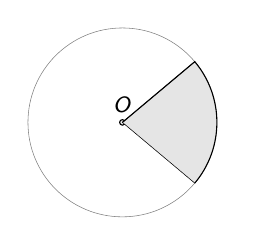
\begin{tikzpicture}[scale=0.6]
    \tkzDefPoints{0/0/O}
    \tkzDefShiftPoint[O](-40:2){H}
    \tkzDefShiftPoint[O](40:2){G}
    \tkzDrawCircle(O,H)
    \tkzLabelPoints[above](O)
    \tkzDrawPoint(O)
    \draw[fill=gray!20] (-40:2) arc (-40:40:2) -- (0,0);
    \tkzDrawSegments(O,G O,H)
    \end{tikzpicture}
\end{minipage}
\end{tcolorbox}
\bigskip 

\begin{example}
What is the area of sector $GPH$? Leave your answers in terms of $\pi$.

\begin{multicols}{2}
\begin{enumerate}[(a)]
    \item \mbox{} 
    \item \mbox{}
\end{enumerate}
\end{multicols}
\begin{minipage}{0.5\textwidth}
    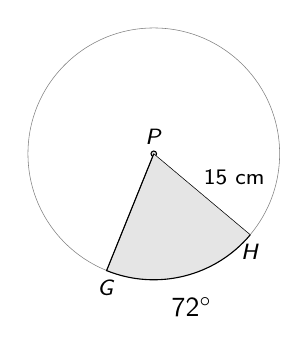
\begin{tikzpicture}[scale=0.8]
    \tkzDefPoints{0/0/P}
    \tkzDefShiftPoint[P](-40:2){H}
    \tkzDefShiftPoint[P](-112:2){G}
    \tkzDrawCircle(P,H)
    \tkzLabelPoints[below](G,H)
    \tkzLabelPoints[above](P)
    \tkzDrawPoint(P)
    \tkzLabelSegment[above right,xshift=-0.1cm](P,H){\footnotesize 15 cm}
    \tkzLabelAngle[pos=2.5](G,P,H){$72^\circ$}
    \draw[fill=gray!20] (-40:2) arc (-40:-112:2) -- (0,0);
    \tkzDrawSegments(P,G P,H)
    \end{tikzpicture}
\end{minipage}
\begin{minipage}{0.4\textwidth}
    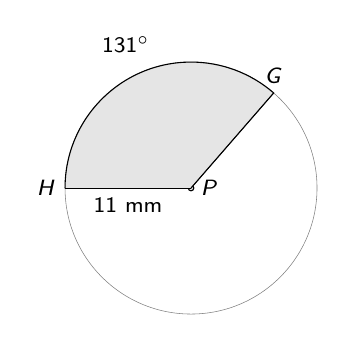
\begin{tikzpicture}[scale=0.8]
    \tkzDefPoints{0/0/P}
    \tkzDefShiftPoint[P](180:2){H}
    \tkzDefShiftPoint[P](49:2){G}
    \tkzDrawCircle(P,H)
    \tkzLabelPoints[left](H)
    \tkzLabelPoints[above](G)
    \tkzLabelPoints[right](P)
    \tkzDrawPoint(P)
    \tkzLabelSegment[below](P,H){\footnotesize 11 mm}
    \tkzLabelAngle[pos=2.5](G,P,H){\footnotesize $131^\circ$}
    \draw[fill=gray!20] (180:2) arc (180:49:2) -- (0,0);
    \tkzDrawSegments(P,H P,G)
    \end{tikzpicture}
\end{minipage}
\end{example}

\vspace{1.75in}

\begin{tcolorbox}[colframe=black!20!white, opacitybacktitle=0.1, coltitle=black, title=\textbf{Segment of a Circle}]
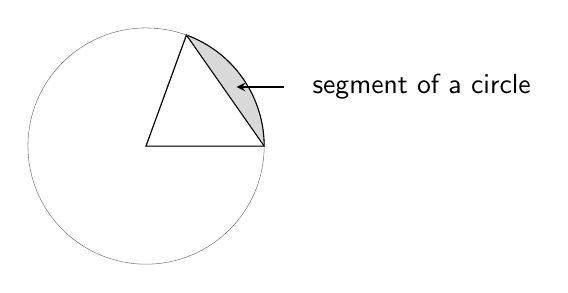
\begin{tikzpicture}
\tkzDefPoints{0/0/O, 1.5/0/A}
\tkzDefShiftPoint[O](70:1.5){B}
\tkzDrawCircle(O,A)
\tkzDrawSegment(A,B)
\draw [fill=gray!30] (0,0) -- (1.5,0) arc (0:70:1.5) -- cycle;
\draw [fill=white!0, color=white!0] (O) -- (A) -- (B) -- cycle;
\draw [black] (O) -- (A) -- (B) -- cycle;
\node at (3.5,0.75) {segment of a circle};
\draw [->, >=stealth] (1.75,0.75) -- (1.15,0.75);
\end{tikzpicture}
\end{tcolorbox}

\newpage 

\begin{center}
\begin{tabular}{p{0.15\linewidth}cp{0.15\linewidth}cp{0.15\linewidth}}
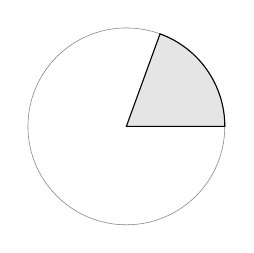
\begin{tikzpicture}
\tkzDefPoints{0/0/O, 1.25/0/A}
\tkzDefShiftPoint[O](70:1.25){B}
\tkzDrawCircle(O,A)
\draw[fill=gray!20] (0,0) -- (1.25,0) arc (0:70:1.25) -- cycle;
\end{tikzpicture}
&
\raisebox{1cm}{$-$}
&
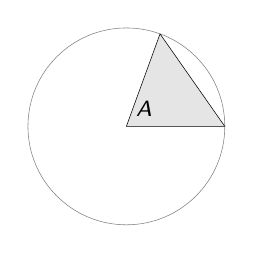
\begin{tikzpicture}
\tkzDefPoints{0/0/O, 1.25/0/A}
\tkzDefShiftPoint[O](70:1.25){B}
\tkzDrawCircle(O,A)
\tkzDrawPolygon[fill=gray!20](A,B,O)
\tkzLabelPoint[above right](O){$A$}
\end{tikzpicture}
&
\raisebox{1cm}{$=$}
&
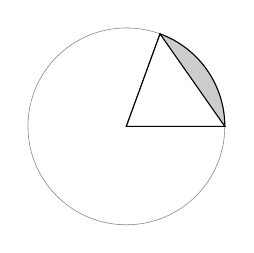
\begin{tikzpicture}
\tkzDefPoints{0/0/O, 1.25/0/A}
\tkzDefShiftPoint[O](70:1.25){B}
\tkzDrawCircle(O,A)
\tkzDrawSegment(A,B)
\draw [fill=gray!40] (0,0) -- (1.25,0) arc (0:70:1.25) -- cycle;
\draw [fill=white!0, color=white!0, dotted] (O) -- (A) -- (B) -- cycle;
\draw [black] (O) -- (A) -- (B) -- cycle;
\end{tikzpicture}   \\[0.1in]
Sector Area &   $-$ &   Triangle Area & $=$ &   Segment Area    \\[0.1in]
&   &   $A = \frac{1}{2}r^2 \sin A$ &   &  \\
\end{tabular}
\end{center}

\vspace{0.25in}

\begin{example}
What is the area of each segment? Round to 2 decimal places.
\begin{multicols}{2}
    \begin{enumerate}[(a)]
        \item \mbox{}
        \item \mbox{}
    \end{enumerate}
\end{multicols}
\begin{minipage}{0.5\textwidth}
    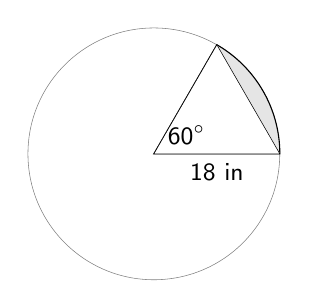
\begin{tikzpicture}[scale=0.8]
    \tkzDefPoints{0/0/C, 2/0/B}
    \tkzDefShiftPoint[C](60:2){A}
    \tkzDrawCircle(C,A)
    \draw [fill=gray!20] (0,0) -- (2,0) arc (0:60:2) -- cycle;
    \tkzDrawPolygon[fill=white](A,B,C)
    \tkzLabelAngle[pos=0.6](B,C,A){\small $60^\circ$}
    \tkzLabelSegment[below](C,B){\small 18 in}
    \end{tikzpicture}
\end{minipage}
\begin{minipage}{0.4\textwidth}
    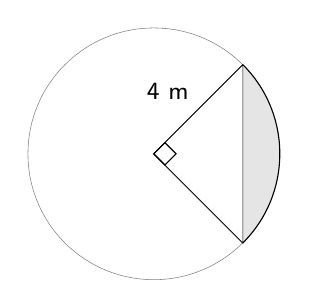
\begin{tikzpicture}[scale=0.8]
    \tkzDefPoints{0/0/Q}
    \tkzDefShiftPoint[Q](45:2){P}
    \tkzDefShiftPoint[Q](-45:2){R}
    \tkzDrawCircle(Q,P)
    \draw[fill=gray!20] (0,0) -- (-45:2) arc (-45:45:2) -- cycle;
    \tkzDrawPolygon[fill=white](Q,P,R)
    \tkzMarkRightAngle(R,Q,P)
    \tkzLabelSegment[above left](Q,P){\small 4 m}
    \end{tikzpicture}
\end{minipage}
\end{example}

\end{document}
